% Preamble
% ---
\documentclass[english]{article}

% Packages
% ---
\usepackage[a4paper, total={6in, 8in}]{geometry}
\usepackage{amsmath} % Advanced math typesetting
\usepackage{bm} %bold math
\usepackage{empheq} % Math left brace
\usepackage[utf8]{inputenc} % Unicode support (Umlauts etc.)
\usepackage[ngerman]{babel} % Change hyphenation rules
\usepackage{hyperref} % Add a link to your document
\usepackage{listings} % Source code formatting and highlighting
\usepackage{graphicx} % Add pictures to your document
\usepackage{subcaption}
\graphicspath{ {img/} }
\usepackage[figurename=Figure]{caption}
\usepackage{url}
%\usepackage{biblatex}
%\addbibresource{bib.bib}


\begin{document}
\selectlanguage{english}


\author{Songbin Liu \\\\ songbinliu@hotmail.com} % The authors name
%\email{}
\title{BPTT for RNN and LSTM} % The title of the document
\date{March 4th, 2018} % Sets date you can remove \today{} and type a date manually
\maketitle{} % Generates title

\begin{abstract}
The training process of RNN/LSTM is not easy to be comprehended. This essay presents a easy way to understand this process.
Firstly, it will explain the BPTT process when training RNN, and the gradient vanishing problem of RNN.  Secondly, it will explain the BPTT
process for LSTM, and how LSTM can handle the gradient vanishing problem better.

\end{abstract}

\section{Introduction}
Recurrent Neural Networks (RNN), especially its variants, such as Long Short Term Memory networks (LSTM) and GRU,
are powerful neural network models. With today's more advanced computation resources, larger volumes of training data,
and better optimization techniques, these models are proved very effective to solve application problems.  There are many
platforms/tools have implemented them, and make them handy for use.

However, it is still useful to understand these models' internal math dynamic process, and how they can be implemented, so that
we can take better use of these models: choose the right model for the application problem, prepare the training data well, and know how to
tune the hyper-parameters.

In this documentation, Section-\ref{sec:rnn} describes the training process of vanilla RNN with some math explanation; 
in addition, the gradient vanishing and exploding problem of vanilla RNN is also explained.  Section-\ref{sec:rnn} describes how to
train the LSTM with math explanation too, and points out how LSTM overcomes the drawback of vanilla RNN.

Note: Because of my humble mathematical background, I will try to explain RNN/LSTM in an intuitive fashion, emphasizing concepts rather than 
mathematical details. In fact, after labeling the layers the unfolded RNN/LSTM properly, the training process is almost the same as training an
ordinary multi-layer feed-forward neural networks.


\section{training RNN with BPTT} \label{sec:rnn}
In this section, the structure of the vanilla RNN is recapped first; second, the process of BPTT to
train this RNN is demonstrated via a simplified example; third, the difficulty of training this vanilla RNN
is explained through an example.

\subsection{Vanilla RNN}
Figure-\ref{fig:vanillaRNN} shows the structure of a vanilla RNN.
\begin{figure}
	\centering
	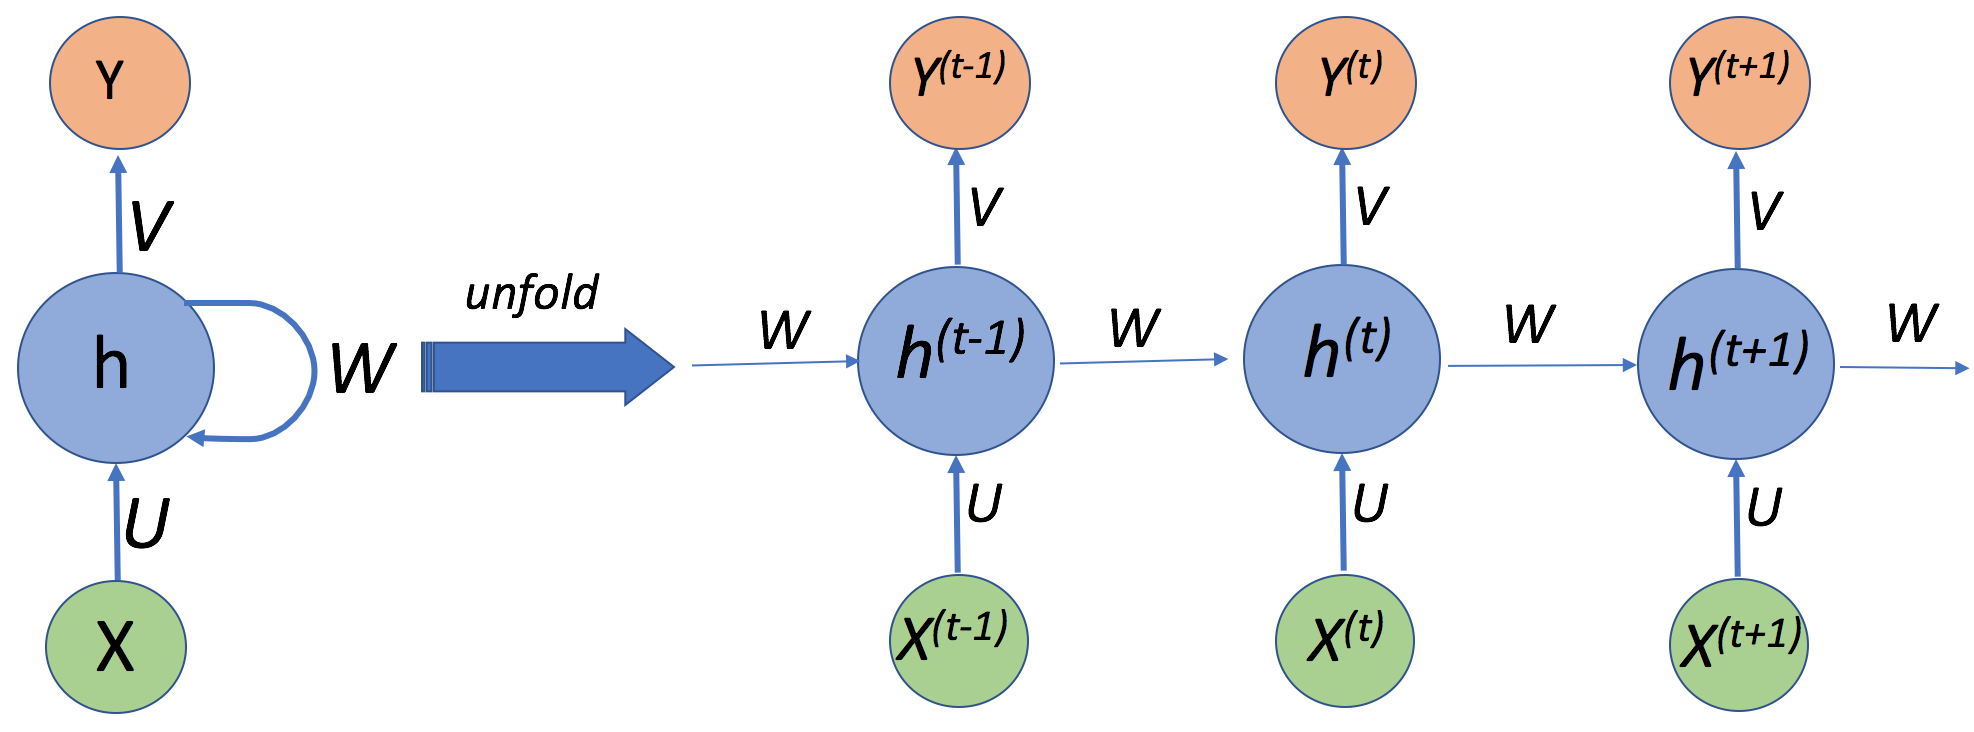
\includegraphics[width=0.8\textwidth]{rnn}
	\caption{Vanilla RNN}
	\label{fig:vanillaRNN}
\end{figure}

\begin{align}
h^{(t)} &= \tanh(Ux^{(t)} + Wh^{(t-1)})\\
y^{(t)} &= softmax(Vh^{(t)})
\end{align}

In this simple RNN, there is an input $x^{(t)}$ and an output $y^{(t)}$ at each time step $t$. $h^{(t)}$ is the hidden state of the RNN at (the end of) time step $t$. The output  $y^{(t)}$ depends on current hidden state. While the current hidden state  $h^{(t)}$  depends not only on current input  $x^{(t)}$ ,
but also depends on previous hidden state  $h^{(t-1)}$ .
The training process will try to learn the parameters: $U$, $W$, and $V$ (and also bias $b$, which is not shown).

\subsection{Training RNN with BPTT}\label{sec:train-rnn}
RNN is trained with the \textit{Backpropagation Through Time (BPTT)} method, which is a variant of the normal \textit{Backpropagation} method for  feed-forward neural networks. When trained with the BPTT method, for each input sequence, RNN is unfolded into a (deep) feed-forward neural network in time dimension (as shown in \ref{fig:vanillaRNN}), the gradients of parameters $U$, $W$ and $V$ are calculated at each layer. 
There are two main differences from the normal \textit{Backpropagation}:  \par
 \textbf{First}, since the parameters $U$, $W$ and $V$ are shared across the steps/layers, these parameters are updated by the sum of the gradients in each step, like the how the shared parameters are updated in Convolutional neural network(CNN). \par
 \textbf{Second}, usually there is an output at each timestep,  so there is one training example at each time step.
 The error of each output is backpropageted to previous steps. In this way, a sequence of  length $T$, will correspond to $T$ overlapped feed-forward neural networks, and the depth of these neural networks is one layer more than previous one.

% Following is a more detailed explanation of this process. 

\subsubsection{Step 1: Unfold the RNN}
For the easy of understanding, the parameters $U$, $W$ and $V$  are labeled with the time step $t$.  In this way, the unfolded RNN looks like a normal
feed-forwad neural network. Figure-\ref{fig:rnn4} shows the resulting neural network of an unfolded RNN of 4 timesteps in total. 
In Figure~\ref{fig:rnn4}, $W^{(t)}$ means the parameter $W$ at timestep (or layer) $t$. $E^{(i)}$ is the error of time step $i$.  Note that even though the parameters $U$, $W$ and $V$  are distinguished by label $t$,  they are treated as one respectively when updating them.

\begin{figure}[htbp]
	\centering
	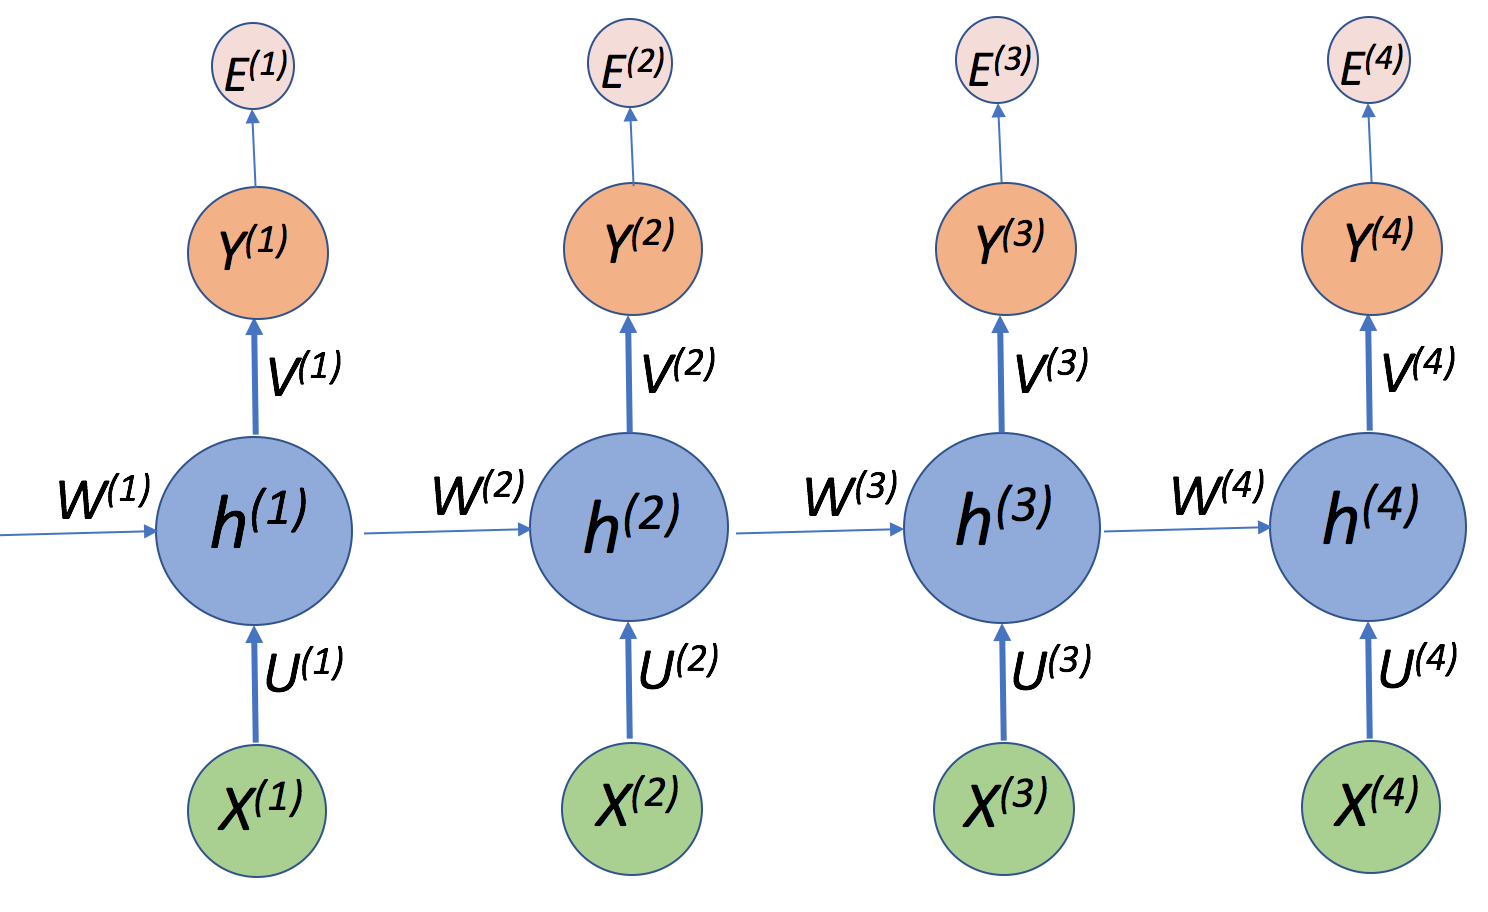
\includegraphics[width=0.7\textwidth]{unfold-rnn}
	\caption{unfolded RNN of 4 time steps}
	\label{fig:rnn4}
\end{figure}


\subsubsection{Step 2: Error Backpropagation for each output}\label{sec:bptt}
Calculate the derivates of the parameters for each output error. The output and input of each timestep is treated as one training example. For this training example, the unfolded RNN is treated as one feed-forward neural network with only one output: the current output, and current output is treated as the last layer of the network.  For example, for timestep $3$, timestep $4$  is ignored, and the previous outputs are also ignored, as is shown in Figure-\ref{fig:step_error}. We only have to calculate the derivates with regard to $V^{(3)}$,  $W^{(1,2,3)}$, and $U^{(1,2,3)}$ for error $E^{(3)}$. Next I will explain how to calculate these derivates for the example in Figure-\ref{fig:step_error}.

\textbf{Firstly}, define $\frac{\partial E^{(3)}}{\partial W^{(j)}}$,  $\frac{\partial E^{(3)}}{\partial U^{(j)}}$, and $\frac{\partial E^{(3)}}{\partial V^{(j)}}$ as the derivates with regard to $W^{(j)}$, $U^{(j)}$ and $V^{(j)}$ for error $E^{(3)}$, where $j \in [1,3]$.

%Secondly, define $\frac{\partial E^{(3)}}{\partial W}$,  $\frac{\partial E^{(3)}}{\partial U}$, and $\frac{\partial E^{(3)}}{\partial V}$ 
\textbf{Secondly}, define $\Delta W^{(3)}$,  $\Delta U^{(3)}$, and $\Delta V^{(3)}$ 
as the derivates with regard to $W$, $U$ and $V$ for error $E^{(3)}$. They are the sum of the derivates of each time step, as is shown in Equation-\ref{eq:delta-t}.

\begin{figure}[htbp]
	\centering
	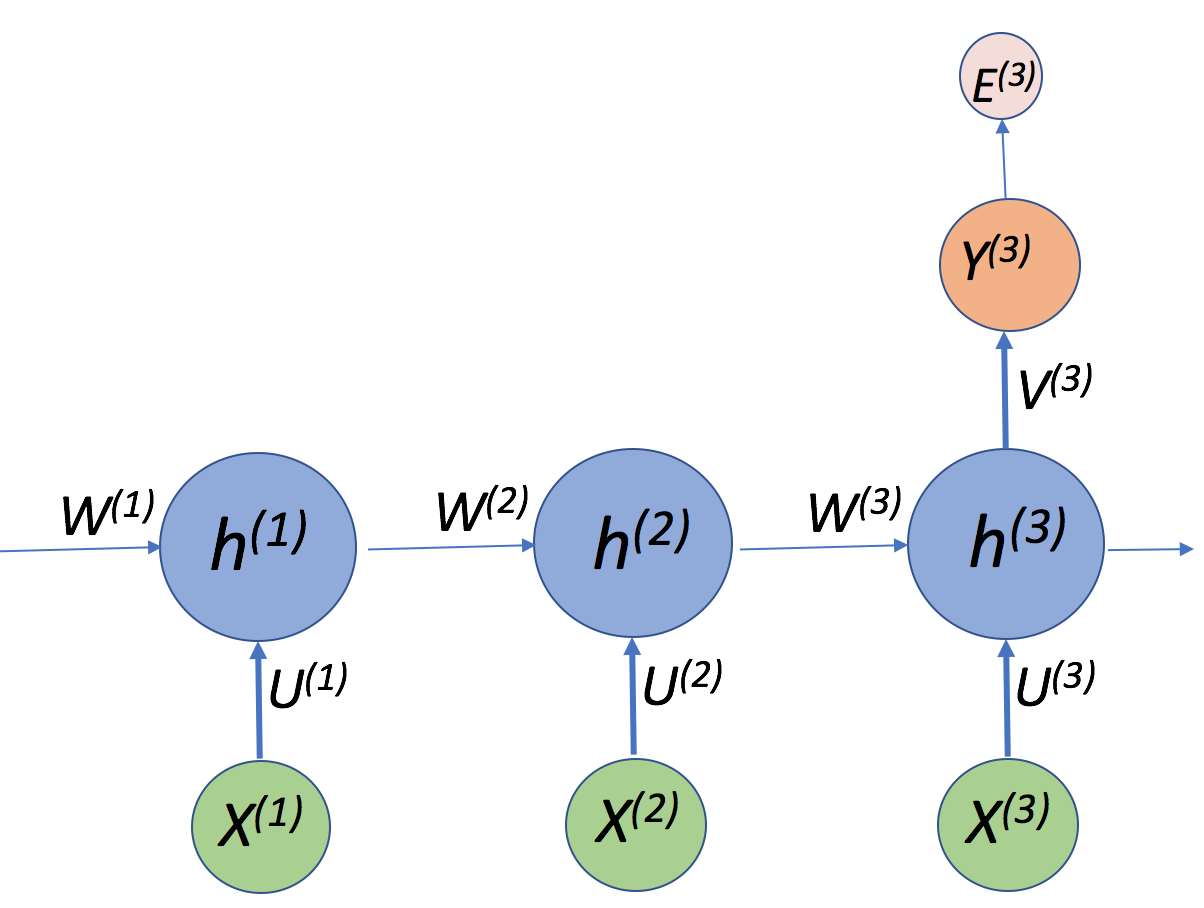
\includegraphics[width=0.7\textwidth]{rnn-example}
	\caption{Calculate the derivates for the output error of timestep 3}
	\label{fig:step_error}
\end{figure}

\begin{equation}\label{eq:delta-t}\begin{cases}
%\begin{empheq}[left=\empheqlbrace]{align}
\Delta W^{(3)} &= \frac{\partial E^{(3)}}{\partial W} = {\sum\limits_{j=1}^3}\frac{\partial E^{(3)}}{\partial W^{(j)}} \\
\Delta U^{(3)} &= \frac{\partial E^{(3)}}{\partial U^{(j)}} = {\sum\limits_{j=1}^3}\frac{\partial E^{(3)}}{\partial U^{(j)}} \\
\Delta V^{(3)} &=\frac{\partial E^{(3)}}{\partial V^{(j)}} = \frac{\partial E^{(3)}}{\partial V^{(j)} }
%\end{empheq}
\end{cases}\end{equation}

%\begin{align}
%\Delta W^{(3)} &= {\sum\limits_{j=1}^3}\frac{\partial E^{(3)}}{\partial W^{(j)}} \\
%\Delta U^{(3)} &= {\sum\limits_{j=1}^3}\frac{\partial E^{(3)}}{\partial U^{(j)}} \\
%\Delta V^{(3)} &=\frac{\partial E^{(3)}}{\partial V^{(j)} }
%\end{align}
 
 To calculate $\Delta W^{(3)}$ and $\Delta U^{(3)}$, we use the similar tricks of \textit{Backpropagation}. Define two auxiliary variables $z^{(t)}$, and  $\delta^{(t)}$ as shown in Equation-\ref{eq:bp}.
 \begin{equation}\label{eq:bp}\begin{cases}
 %\begin{align} 
 z^{(t)} &= U^{(t)} x^{(t)} + W^{(t)} h^{(t-1)}\\
 \delta^{(t)} &= \frac{\partial E^{(3)}}{\partial z^{(t)}}
% \end{align}
 \end{cases}\end{equation}
 
 
 With equation-\ref{eq:bp},  $\frac{\partial E^{(3)}}{\partial W^{(j)}}$,  $\frac{\partial E^{(3)}}{\partial U^{(j)}}$  can be calculated by Equation-\ref{eq:bp-2}.
 \begin{equation}\label{eq:bp-2}\begin{cases}
 \frac{\partial E^{(3)}}{\partial W^{(j)}} &= \frac{\partial E^{(3)}}{\partial z^{(j)}} \frac{\partial z^{(j)}}{\partial W^{(j)}}  = \delta^{(j)} h^{(j-1)}\\
\frac{\partial E^{(3)}}{\partial U^{(j)}} &= \frac{\partial E^{(3)}}{\partial z^{(j)}} \frac{\partial z^{(j)}}{\partial U^{(j)}}  = \delta^{(j)} x^{(j)}\\
 \end{cases}\end{equation}
 While $\delta^{(j)}$ can be calculated by the chain rule, as is shown in Equation-\ref{eq:bp-3}.
 \begin{equation}\label{eq:bp-3}
  \delta^{(j)} = \frac{\partial E^{(3)}}{\partial z^{(j+1)}} \frac{\partial z^{(j+1)}}{\partial z^{(j)}} =\delta^{(j+1)} W^{(j+1)} tanh^{\prime}(z^{(j)})
 \end{equation}
 
 
 In summary,  we can \textbf{use the following backpropagation process to calculate the derivates for error $E^{(3)}$}, which is shown in 
 Equation-\ref{eq:delta-t2}.
 
 \begin{equation}\label{eq:delta-t2}\begin{cases}
 %\begin{align}
 \delta^{(j)} &= \delta^{(j+1)} W^{(j+1)} tanh^{\prime}(z^{(j)}) \\
\Delta W^{(3)} &= {\sum\limits_{j=1}^3}\delta^{(j)}\frac{\partial z^{(j)}}{\partial W^{(j)}} = {\sum\limits_{j=1}^3}\delta^{(j)}h^{(j-1)}\\
\Delta U^{(3)} &= {\sum\limits_{j=1}^3}\delta^{(j)}\frac{\partial z^{(j)}}{\partial W^{(j)}} = {\sum\limits_{j=1}^3}\delta^{(j)}x^{(j)} \\
%\end{align}
\end{cases}\end{equation}


\subsubsection{Step 3: Average up the derivatives for the sequence}
% Calculate the derivates of the parameters of current input sequence.
As mentioned earlier, each timestep is a training example, so there are $T$ training examples for a training sequence of length $T+1$.
These training examples can be treated as a mini-batch.  Thus, the derivates of $W$, $U$ and $V$ for one sequence (or several sequences) are the
average of the derivates for each output, as is shown in Equation-\ref{eq:batch-1}.
 
 \begin{equation}\label{eq:batch-1}\begin{cases}
%\begin{align}
\Delta W &=  \frac{1}{T}\sum\limits_{i=1}^T\Delta W^{(i)}\\
\Delta U &=  \frac{1}{T}\sum\limits_{i=1}^T\Delta U^{(i)}\\
\Delta V &=  \frac{1}{T}\sum\limits_{i=1}^T\frac{\partial E^{(i)}}{\partial V^{(j)}}
%\end{align}
\end{cases}\end{equation}
Where, $T+1$ is the length of the input training sequence, $E^{(i)}$ is the error of time step $i$.

\subsubsection{Step 4: update the parameters} 
After all the derivates of the parameters of current input sequence (or sequence batch) have been calculated, we can update the parameters with Equations-\ref{eq:update}.
\begin{equation}\label{eq:update}\begin{cases}
W &= W  - \lambda \Delta W\\
U &= U - \lambda \Delta U\\
V &= V - \lambda \Delta V\\
\end{cases}\end{equation}
where $\lambda$ is the learning rate. There are various ways to set a proper learning rate for each weight.


\subsection{Gradient vanishing and exploding of RNN}
The vanilla RNN model looks very promising for sequential problems, but it did not work well in application.  
This is because of the gradient vanishing and exploding problem during the training process, it is very difficult to train the RNN model in practice.

\begin{align}\label{eq:bp-4}
%\delta^{(j-1)} &= \delta^{(j)} W^{(j)} tanh^{\prime}(z^{(j-1)})\\
\delta^{(1)} &= \delta^{(4)} W^{(4)} tanh^{\prime}(z^{(3)}) W^{(3)} tanh^{\prime}(z^{(2)}) W^{(2)} tanh^{\prime}(z^{(1)})
\end{align}


How does the gradient vanishing or exploding problem happen? Here is an example. 
Suppose to backpropagate the output error of timestep 4 to timestep 1. As explained in section-\ref{sec:bptt},  to calculate $\frac{\partial E^{(4)}}{\partial W^{(1)}}$,  $\frac{\partial E^{(4)}}{\partial U^{(1)}}$, we need to get $\delta^{(1)}$ according to equations-\ref{eq:bp-2}. And according to equation-\ref{eq:bp-3}, $\delta^{(1)}$ can be obtained by equation-\ref{eq:bp-4}. If the $W^{(j)}tanh^{\prime}(z^{(j-1)})$ terms are greater than 1, then gradient exploding can happen, and will cause numerical overflow. If \textbf{the $W^{(j)}tanh^{\prime}(z^{(j-1)})$ terms  are smaller than 1}, 
then the gradient tends to be vanishing, which means the error can only be backpropagated to nearby steps (it can only have very short memory of very nearby inputs). 

\begin{figure}[htbp]
	\begin{subfigure}{0.5\textwidth}
  		\centering
 		 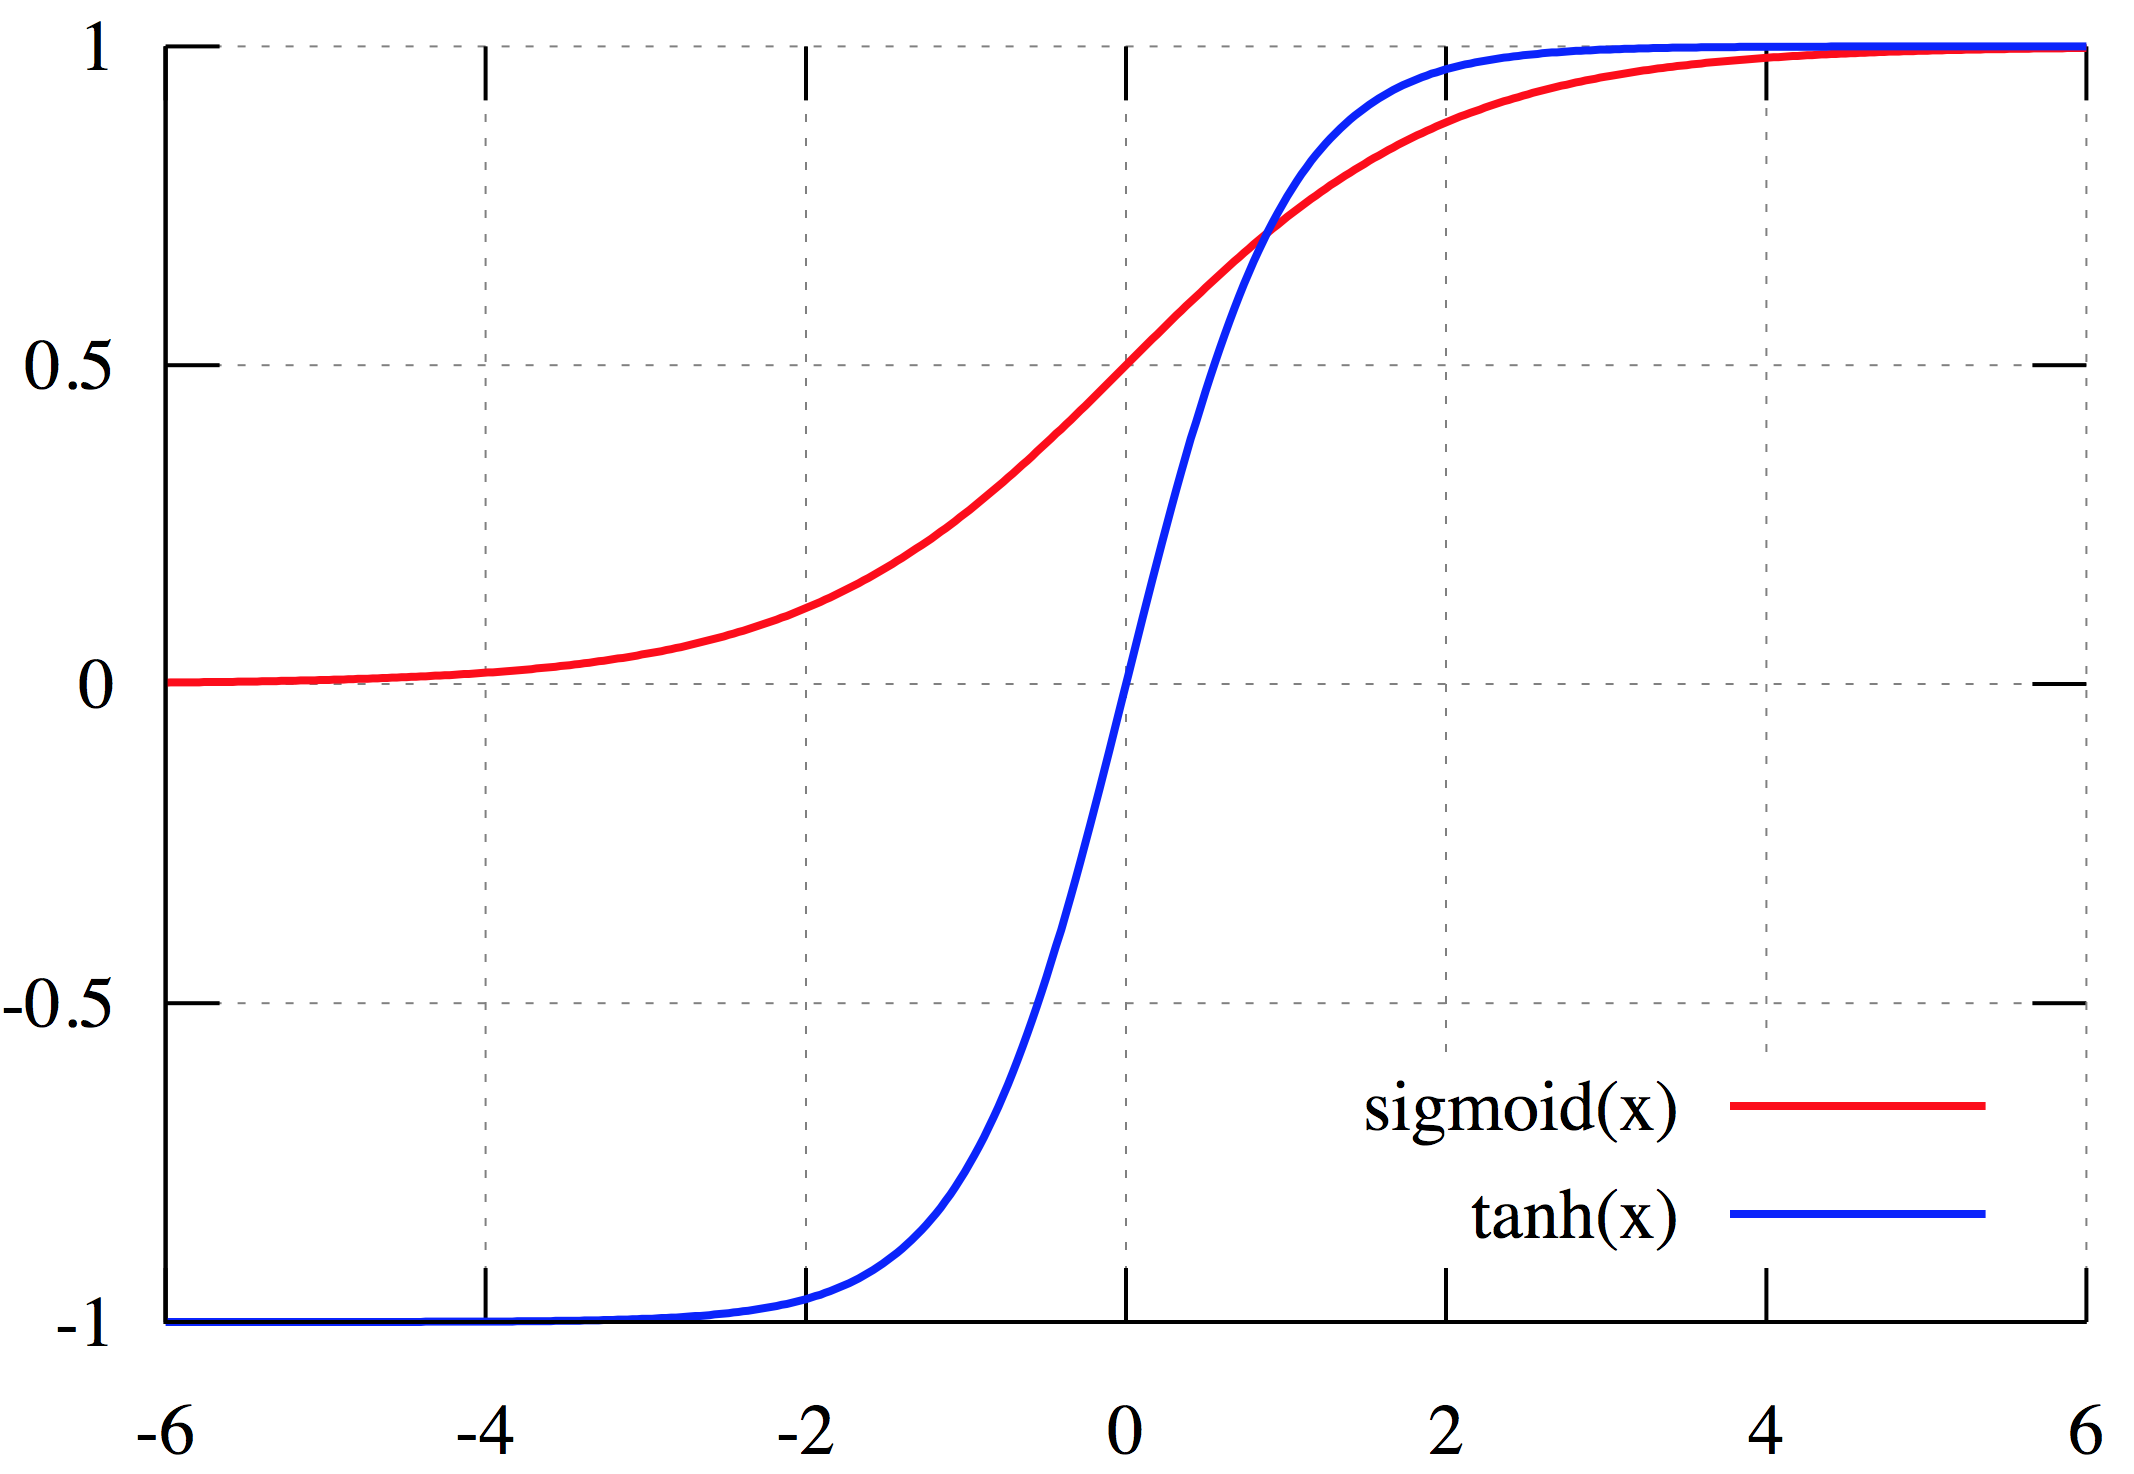
\includegraphics[width=0.95\linewidth]{active}
  		\caption{Activation functions}
  		\label{fig:nnet-active}
	\end{subfigure}
	\begin{subfigure}{0.5\textwidth}
 	 	\centering
 	 	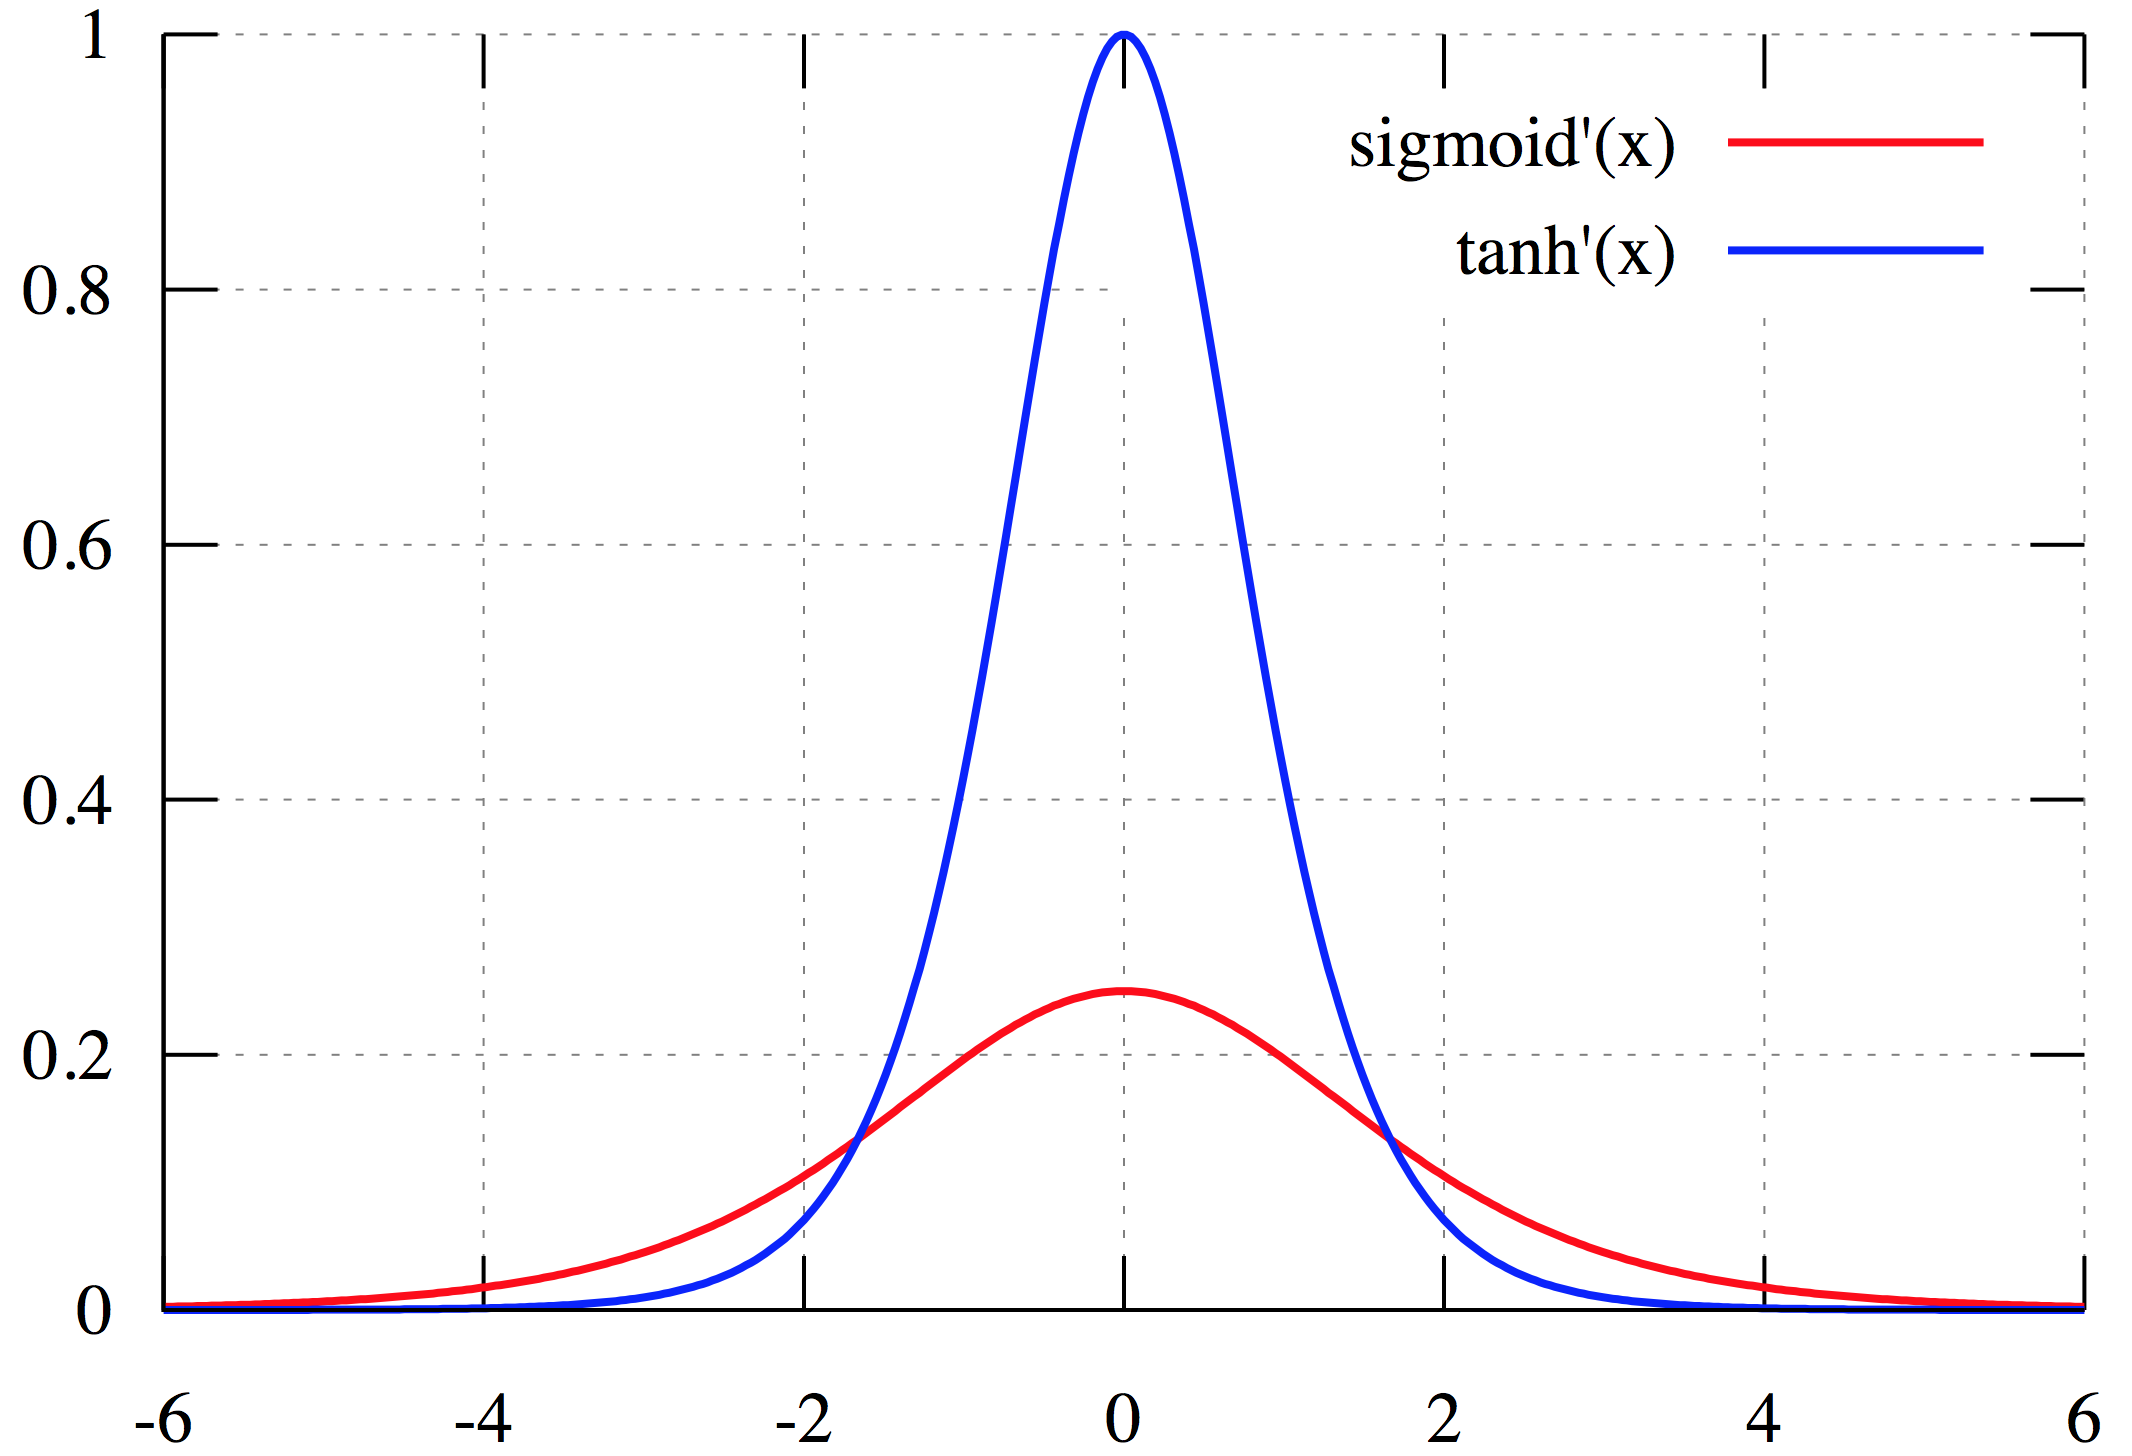
\includegraphics[width=0.95\linewidth]{derivate}
 	 	\caption{Derivatives of the activation functions}
 	 	\label{fig:nnet-derivate}
	\end{subfigure}
	\caption{$sigmoid$ and $tanh$ functions and their derivatives}
	\label{fig:nnet-functions}
\end{figure}


Usually, the gradient exploding problem can be handled by gradient clipping, and won't be a big problem for training RNN. 
The gradient vanishing problem is the major obstacle when training RNN. The gradient vanishing can happen very likely. As shown in Figure-\ref{fig:nnet-derivate}, the derivatives of the two commonly used activation functions $sigmoid$ and $tanh$ are very near to zero. Their derivatives are only significantly larger than zero  in a very small interval (for example, $\tanh^{\prime}(-3) \approx 0.01$, $sigmoid^{\prime}(-3) \approx 0.047$). Even with very carefully set of the initial weights, the gradient still can get decreased to zero in  exponential order with the number of layers increase.

\section{LSTM}
Long Short Term Memory network (LSTM)  is a special kind of RNN, and is capable of learning long-term dependencies. It can handle the gradient vanishing problem much better, and are widely used in practice. There are several variants of LSTM, but in this section, we focus on the simplest one.
It has a cell state, and a hidden state, three gates: forget gates, input gates, and output gates. These gates are controlled by current input and the hidden state(no peephole connection from the cell state).
 

\subsection{Structure of LSTM}
Define $x^{(t)}$ is the input of timestep $t$, $C^{(t)}$ is the cell state, $h^{(t)}$ is the hidden state,  $y^{(t)}$ is the output.
The forward process to update these values is shown in Equations-\ref{eq:input-gate}--\ref{eq:output}.


\begin{empheq}[left=\empheqlbrace]{align}
\label{eq:input-gate}
i^{(t)} &= \sigma(W_i \cdot [h^{(t-1)}, x^{(t)}]) \\
\label{eq:input-value}
A^{(t)} &= \tanh(W_a \cdot [h^{(t-1)}, x^{(t)}])\\
\label{eq:forget-gate}
f^{(t)} &= \sigma(W_f \cdot [h^{(t-1)}, x^{(t)}]) \\
\label{eq:update-cell}
C^{(t)} &= f^{(t)}  \cdot C^{(t-1)} + i^{(t)}  \cdot A^{(t)} \\
\label{eq:output-gate}
o^{(t)} &= \sigma(W_o \cdot [h^{(t-1)}, x^{(t)}]) \\
\label{eq:update-hidden}
h^{(t)} &= o^{(t)} \cdot \tanh(C^{(t)})\\
\label{eq:output}
y^{(t)} &= softmax(V \cdot h^{(t)})
\end{empheq}

\textbf{Firstly},update the cell state(Equation-\ref{eq:update-cell}) with the input gate(Equation-\ref{eq:input-gate}), 
input value(Equation-\ref{eq:input-value}), forget gate(Equation-\ref{eq:forget-gate}), and previous cell state;


\textbf{Secondly}, update hidden state(Equation-\ref{eq:update-hidden}) with the new cell state and output gate(Equation-\ref{eq:output-gate});

\textbf{Lastly}, calculate the output based on the new hidden state(Equation-\ref{eq:output});

The training process will try to learn the parameters $W_i, W_a, W_f, W_o$, and $V$ (and also the biases). As a comparison, the vanilla RNN
only has $W_a$ and $V$.

\subsection{Training LSTM}
BPTT is also used to train LSTM neural networks. The process of training LSTM is similar to the process for a vanilla RNN as is shown in Section~\ref{sec:train-rnn}

\begin{figure}[htbp]
	\centering
	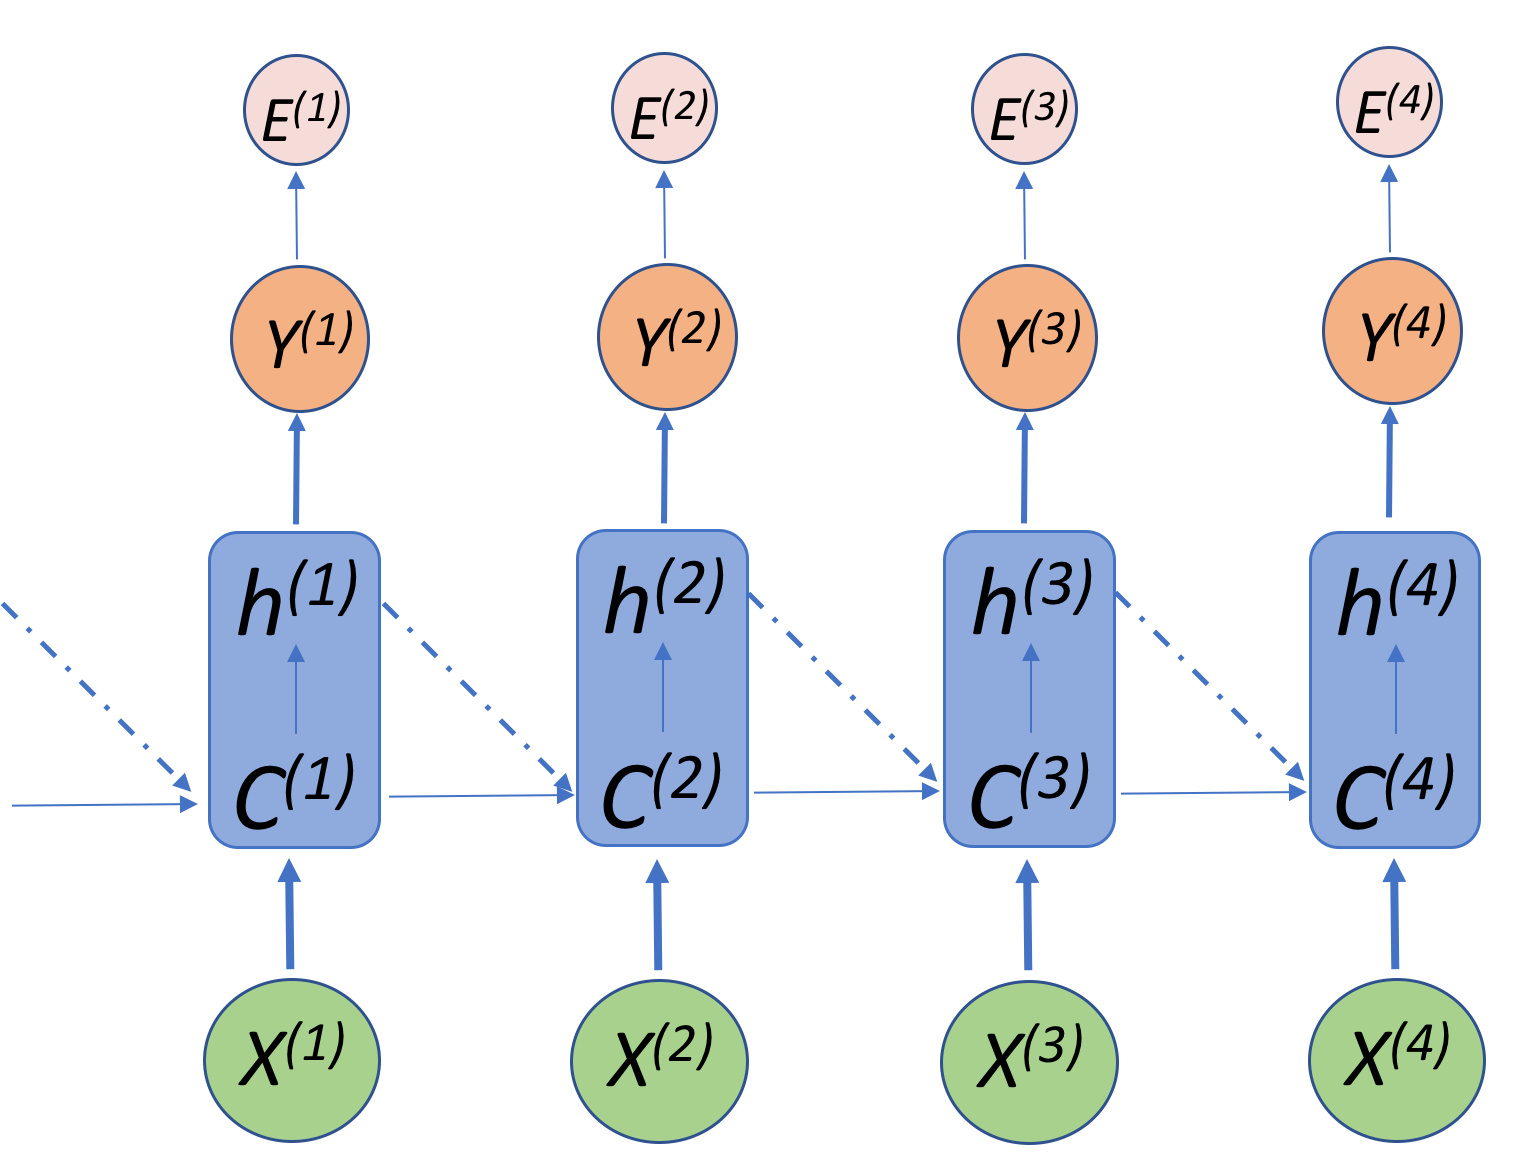
\includegraphics[width=0.65\textwidth, keepaspectratio]{lstm}
	\caption{Unfolded LSTM with length of 4}
	\label{fig:lstm}
\end{figure}


\textbf{Step 1}: Unfold the input training sequence into a feed-forward neural network, as shown in Figure~\ref{fig:lstm};

\textbf{Step 2}: For each output, treat the output and all the steps ( or layers) before that output as a feed-forward neural network,
and calculate the derivates for the parameters with regard to this output error. Sum up the derivates for each parameter;

\textbf{Step 3}: Average the derivatives for the all the outputs for the input sequence;

\textbf{Step 4}: Update the parameters with the averaged derivative for each parameter with a proper learning rate.

The only difference from the vanilla RNN is in \textbf{Step 2}, which will be discussed in detail in following subsection.

\subsubsection{Step 1: Unfold the LSTM}
Similar to RNN, the unfolded LSTM looks like a normal feed-forward neural network, and the parameters are also distinguished with timestep $t$, as shown in Figure~\ref{fig:lstm}. 
However, LSTM has more parameters, and the internal process is much more complicated than that of RNN.

\subsubsection{Step 2: Calculate the derivates for one output error}
The output and input of each timestep of LSTM is also treated as one training example. For each training example, the unfolded LSTM is treated as one feed-forward neural network with only one output: the current output, and current output is treated as the last layer of the network.  
For example, when calculate the derivatives for the output error of timestep $3$, timestep $4$  is ignored, and the previous outputs are also ignored, as is shown in Figure-\ref{fig:lstm-one}. We only have to calculate the derivates with regard to $W^{(1,2,3)}_f$, $W^{(1,2,3)}_i$, $W^{(1,2,3)}_a$, $W^{(1,2,3)}_o$, and $V^{(3)}$ for error $E^{(3)}$. Next will explain how to calculate these derivates with the example in Figure-\ref{fig:lstm-one}.

\begin{figure}[htbp]
	\centering
	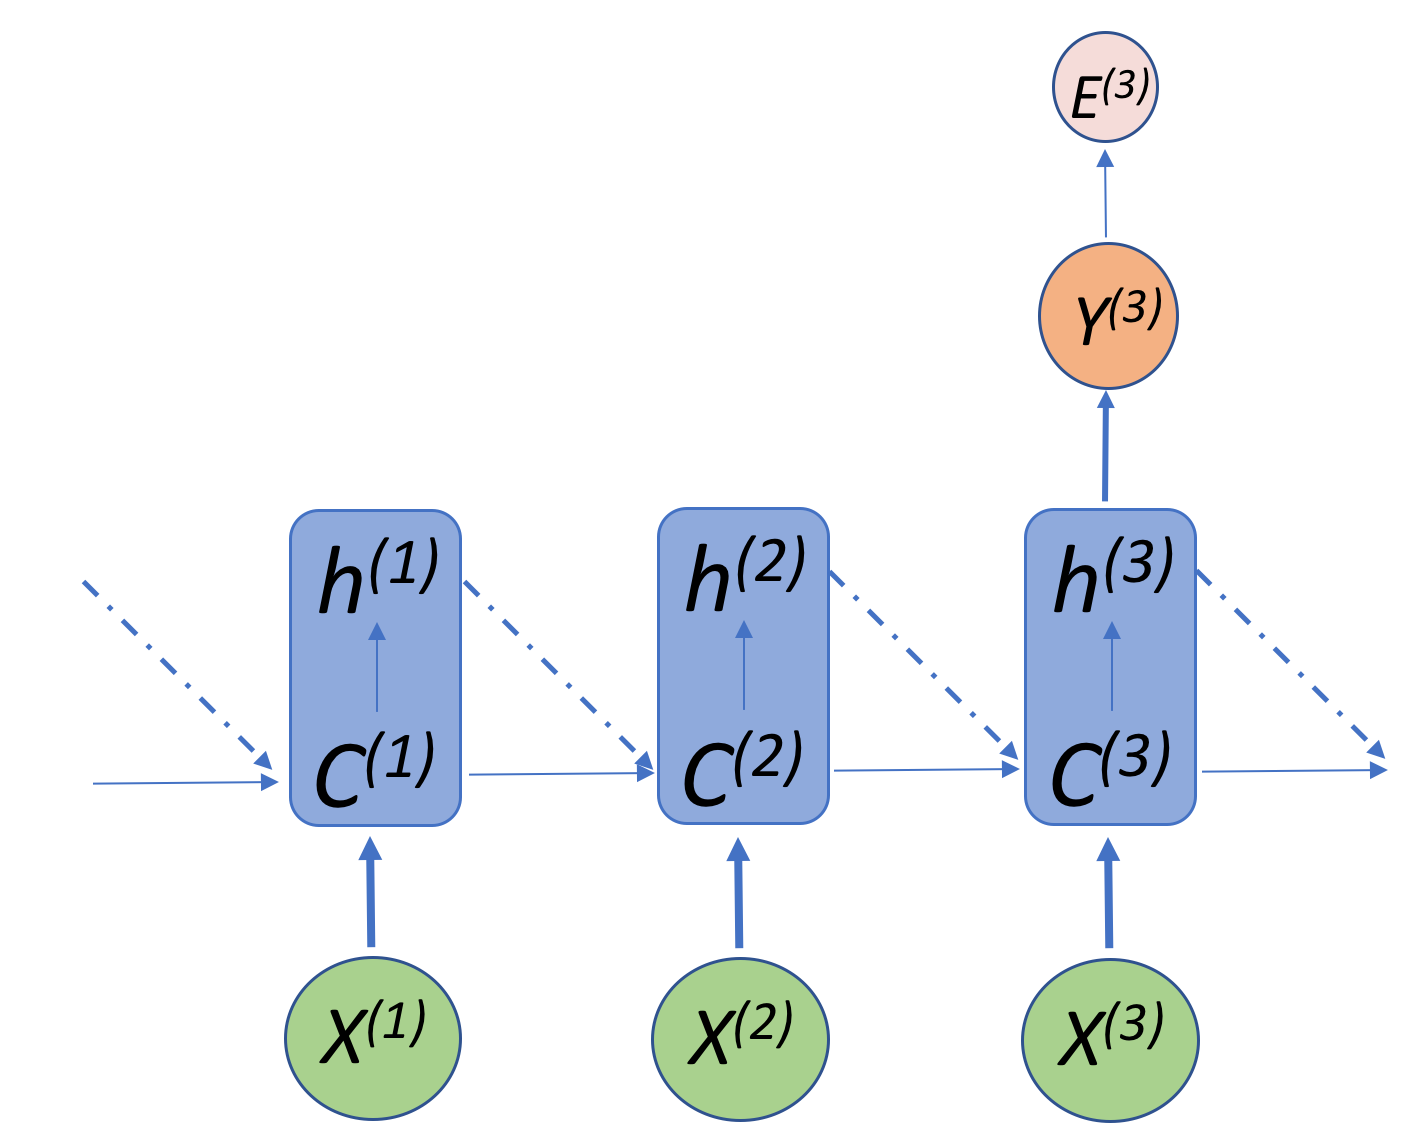
\includegraphics[width=0.65\textwidth, keepaspectratio]{lstm-one}
	\caption{Calculate the derivates for the output error of timestep 3 in LSTM}
	\label{fig:lstm-one}
\end{figure}


\textbf{Firstly}, define $\frac{\partial E^{(3)}}{\partial W^{(j)}_f}$,  $\frac{\partial E^{(3)}}{\partial W^{(j)}_i}$, $\frac{\partial E^{(3)}}{\partial W^{(j)}_a}$,  $\frac{\partial E^{(3)}}{\partial W^{(j)}_o}$, and $\frac{\partial E^{(3)}}{\partial V^{(j)}}$ as the derivates with regard to $W^{(1,2,3)}_f$, $W^{(1,2,3)}_i$, $W^{(1,2,3)}_a$, $W^{(1,2,3)}_o$, and $V^{(3)}$  for error $E^{(3)}$.

%Secondly, define $\frac{\partial E^{(3)}}{\partial W}$,  $\frac{\partial E^{(3)}}{\partial U}$, and $\frac{\partial E^{(3)}}{\partial V}$ 
\textbf{Secondly}, define $\Delta W^{(3)}_f$,  $\Delta W^{(3)}_i$, $\Delta W^{(3)}_a$, $\Delta W^{(3)}_o$, and $\Delta V^{(3)}$ 
as the derivates with regard to $W_f, W_i, W_a, W_o$,  and $V$ for error $E^{(3)}$. They are the sum of the derivates of each time step, as is shown in Equation-\ref{eq:lstm-delta-3}.


\begin{equation}\label{eq:lstm-delta-3}\begin{cases}
%\begin{empheq}[left=\empheqlbrace]{align}
\Delta W^{(3)}_f &= \frac{\partial E^{(3)}}{\partial W_f} = {\sum\limits_{j=1}^3}\frac{\partial E^{(3)}}{\partial W^{(j)}_f} \\
\Delta W^{(3)}_i &= \frac{\partial E^{(3)}}{\partial W_i} = {\sum\limits_{j=1}^3}\frac{\partial E^{(3)}}{\partial W^{(j)}_i} \\
\Delta W^{(3)}_a &= \frac{\partial E^{(3)}}{\partial W_a} = {\sum\limits_{j=1}^3}\frac{\partial E^{(3)}}{\partial W^{(j)}_a} \\
\Delta W^{(3)}_o &= \frac{\partial E^{(3)}}{\partial W_o} = {\sum\limits_{j=1}^3}\frac{\partial E^{(3)}}{\partial W^{(j)}_o} \\
\Delta V^{(3)} &=\frac{\partial E^{(3)}}{\partial V^{(j)}} = \frac{\partial E^{(3)}}{\partial V^{(j)} }
%\end{empheq}
\end{cases}\end{equation}

\textit{Backpropagation} method is used to calculate $\Delta W^{(3)}_f$,  $\Delta W^{(3)}_i$, $\Delta W^{(3)}_a$, and $\Delta W^{(3)}_o$. Here define one auxiliary variable $\delta^{(j)}$ as the derivative with regard to $C^{(j)}$, as is shown in Equation-\ref{eq:lstm-delta}. 
\begin{equation}\label{eq:lstm-delta}
\delta^{(j)} = \frac{\partial E^{(3)}}{\partial C^{(j)}}
\end{equation}

Suppose, the value of $\delta^{(j)}$  is available, then $\frac{\partial E^{(3)}}{\partial W^{(j)}_f}$ can be calculate via Equation-\ref{eq:delta-wf}, according to Equation-\ref{eq:update-cell} and \ref{eq:forget-gate}. 

\begin{equation}\label{eq:delta-wf}
\begin{split}
\frac{\partial E^{(3)}}{\partial W^{(j)}_f} &= \frac{\partial E^{(3)}}{\partial C^{(j)}_f} \cdot \frac{\partial C^{(j)}}{\partial W^{(j)}_f}  \\                                                       
                                                             &= \delta^{(j)} \cdot \frac{\partial C^{(j)}}{\partial W^{(j)}_f} \\
   &= \delta^{(j)} \cdot  \sigma^{\prime}(W_f \cdot [h^{(j-1)}, x^{(j)}]) \cdot ([h^{(j-1)}, x^{(j)}]) \cdot C^{(j-1)}  \\
\end{split}                                                             
\end{equation}

Similarly, $\frac{\partial E^{(3)}}{\partial W^{(j)}_i}$ and $\frac{\partial E^{(3)}}{\partial W^{(j)}_a}$ can be calculate with $\delta^{(j)}$. 
However, it is $C^{(j+1)}$,  not $C^{(j)}$ depends on $W^{(j)}_o$ (via $h^{(j)}$),  so the computation of $\frac{\partial E^{(3)}}{\partial W^{(j)}_o}$ is 
kind of more complicated, and will be addressed at the end of this section.


 \begin{equation}\label{eq:hc-lstm}
    \tau^{(j)} = \frac{\partial h^{(j)}}{\partial C^{(j)}} = o^{(j)} \cdot \tanh'(C^{(j)})\\
\end{equation}


Next, we will give the backward recurrence formula to compute $\delta^{(j)}$ based on $\delta^{(j+1)}$ for LSTM. 
%Equation-\ref{eq:update-cell} defines the relationship between $C^{(j)}$ and $C^{(j-1)}$.
It should be noted that in Equation-\ref{eq:update-cell}, $f^{(j)}$, $i^{(j)}$ and $A^{(j)}$ also depend on $C^{(j-1)}$ via variable $h^{(j-1)}$. For the easy of notation, another auxiliary variable $\tau^{(j)}$ is defined as the derivative of $h^{(j)}$ with regard to $C^{(j)}$. Based on Equation-\ref{eq:update-hidden}, $\tau^{(j)}$ can be calculate with Equation-\ref{eq:hc-lstm}.

 \begin{equation}\label{eq:delta-lstm-recurrence}
 \begin{split}
    \delta^{(j)} &= \frac{\partial E^{(3)}}{\partial C^{(j)}} \\
                     &=  \frac{\partial E^{(3)}}{\partial C^{(j+1)}}  \frac{\partial C^{(j+1)}}{\partial C^{(j)}} \\
                     &= \delta^{(j+1)} \cdot  \frac{\partial [f^{(j+1)} \cdot C^{(j)} + i^{(j+1)}  \cdot A^{(j+1)}]}{\partial C^{(j)}} \\
                     &= \delta^{(j+1)} \cdot (f^{(j+1)}  + \frac{\partial f^{(j+1)}}{\partial h^{(j)}}\frac{\partial h^{(j)}}{\partial C^{(j)}} \cdot C^{(j)} +
                         \frac{\partial i^{(j+1)}}{\partial h^{(j)}}\frac{\partial h^{(j)}}{\partial C^{(j)}} \cdot A^{(j+1)} +
                         i^{(j+1)}  \cdot \frac{\partial A^{(j+1)}}{\partial h^{(j)}}\frac{\partial h^{(j)}}{\partial C^{(j)}})\\
                    &= \pmb{\delta^{(j+1)} \cdot f^{(j+1)} } + 
                           \delta^{(j+1)} \tau^{(j)} \cdot (\frac{\partial f^{(j+1)}}{\partial h^{(j)}} \cdot C^{(j)} +
                                                                         \frac{\partial i^{(j+1)}}{\partial h^{(j)}} \cdot A^{(j+1)} +
                                                                        i^{(j+1)} \cdot \frac{\partial A^{(j+1)}}{\partial h^{(j)}})\\
 \end{split}                       
\end{equation}

In Equation-\ref{eq:delta-lstm-recurrence}, the computation of $\frac{\partial f^{(j+1)}}{\partial h^{(j)}}$, $\frac{\partial i^{(j+1)}}{\partial h^{(j)}}$, and 
$\frac{\partial A^{(j+1)}}{\partial h^{(j)}}$ are very simple. For example, based on Equation-\ref{eq:input-gate}, 
$\frac{\partial f^{(j+1)}}{\partial h^{(j)}}$ can be calculated with Equation-\ref{eq:forget-delta}.

\begin{equation}\label{eq:forget-delta}
     \frac{\partial f^{(j+1)}}{\partial h^{(j)}} = \sigma^{\prime}(W_i \cdot [h^{(j)}, x^{(j+1)}]) \cdot W_{i,h}
\end{equation}
where $W_{i,h}$ is the part which acts on hidden state $h^{(j)}$ of the whole input gate weight $W_i$ .

In summary, with Equation-\ref{eq:delta-lstm-recurrence},  $\delta^{(j)}$ can be computed; 
with Equation-\ref{eq:delta-wf} and Equations-\ref{eq:lstm-delta-3},  $\Delta W^{(3)}_f$,  $\Delta W^{(3)}_i$, $\Delta W^{(3)}_a$ can be computed from $\delta^{(j)}$. (The computation of $\Delta W^{(3)}_o$ is described in next subsection).

\subsubsection{Step 3: Average up the derivatives for the sequence}
Similar to RNN, each timestep is a training example, so there are $T$ training examples for a training sequence of length $T+1$.
These training examples can be treated as a mini-batch.  Thus, the derivatives of $W$, $U$ and $V$ for one sequence (or several sequences) are the
average of the derivates for each output, as is shown in Equation-\ref{eq:lstm-batch}.
 
 \begin{equation}\label{eq:lstm-batch}\begin{cases}
%\begin{align}
\Delta W_i &=  \frac{1}{T}\sum\limits_{i=1}^T\Delta W^{(i)}_i\\
\Delta W_a&=  \frac{1}{T}\sum\limits_{i=1}^T\Delta W^{(i)}_a\\
\Delta W_f &=  \frac{1}{T}\sum\limits_{i=1}^T\Delta W^{(i)}_f\\
\Delta W_o &=  \frac{1}{T}\sum\limits_{i=1}^T\Delta W^{(i)}_o\\
\Delta V &=  \frac{1}{T}\sum\limits_{i=1}^T\frac{\partial E^{(i)}}{\partial V^{(j)}}
%\end{align}
\end{cases}\end{equation}
Where, $T+1$ is the length of the input training sequence, $E^{(i)}$ is the error of time step $i$.
 
\subsubsection{Step 4: update the parameters} 
After all the derivates of the parameters of current input sequence (or sequence batch) have been calculated, we can update the parameters with Equations-\ref{eq:lstm-update}.
\begin{equation}\label{eq:lstm-update}\begin{cases}
W_i &= W_i  - \lambda \Delta W_i\\
W_a &= W_a  - \lambda \Delta W_a\\
W_f &= W_f  - \lambda \Delta W_f\\
W_o &= W_o  - \lambda \Delta W_o\\
V &= V - \lambda \Delta V\\
\end{cases}\end{equation}
where $\lambda$ is the learning rate. 

\subsubsection{Note:  calculate the derivative for $W_o$} 
TODO

\subsection{How LSTM handles the gradient vanishing problem}
As mentioned earlier, LSTM can handle the gradient vanishing problem much better than vanilla RNN.  For the easy of explanation, let's simplify
Equation-\ref{eq:delta-lstm-recurrence} further. In the end of Equation-\ref{eq:delta-lstm-recurrence},  $\delta^{(j)}$ is the sum of two parts.  According 
to Equation-\ref{eq:forget-delta}, and Equation-\ref{eq:hc-lstm}, the later part of Equation-\ref{eq:delta-lstm-recurrence} contains a product of $tanh'(C) \cdot sigmoid'(z)$. Based on the analysis of the Figure-\ref{fig:nnet-derivate}, $tanh'(C) \cdot sigmoid'(z)$ is likely two orders smaller than 1. 
So for here, for analysis we can ignore the later part of Equation-\ref{eq:delta-lstm-recurrence}, and get $\delta^{(j)}$ for LSTM approximately via 
Equation-\ref{eq:lstm-delta-simple}.

\begin{equation}\label{eq:lstm-delta-simple}
\delta^{(j)}_{lstm}  \approx \delta^{(j+1)}_{lstm} \cdot f^{(j+1)} = \delta^{(j+1)}_{lstm} \cdot \sigma(z_f) \\
\end{equation}

As comparison, the $\delta^{(j)}$ for RNN of Equation-\ref{eq:bp-3} can be re-written in Equation-\ref{eq:rnn-delta-label}.
\begin{equation}\label{eq:rnn-delta-label}
 \delta^{(j)}_{rnn} = \delta^{(j+1)}_{rnn} \cdot W^{(j+1)} \cdot tanh^{\prime}(z^{(j)})\\
\end{equation}

The main reason that $\delta^{(j)}_{rnn}$ will be shrinking very fast because of the $tanh^{\prime}(z^{(j)})$ term in Equation-\ref{eq:rnn-delta-label};
however, $\delta^{(j)}_{lstm}$ only has the $\sigma(z_f)$ term, which is much better. As is shown in Figure-\ref{fig:compare}, $tanh^{\prime}(x)$ 
can be significantly larger than zero only in the interval $[-4, 4]$; on the other hand, $\sigma(x)$  can be significantly larger than zero in a much larger
interval $[-4, +\infty]$. Thus $\delta^{(j)}_{lstm}$ will shrink much slower than $\delta^{(j)}_{rnn}$. In other words, the cell state of LSTM can have much
longer memory for previous inputs.

\begin{figure}[htbp]
	\centering
	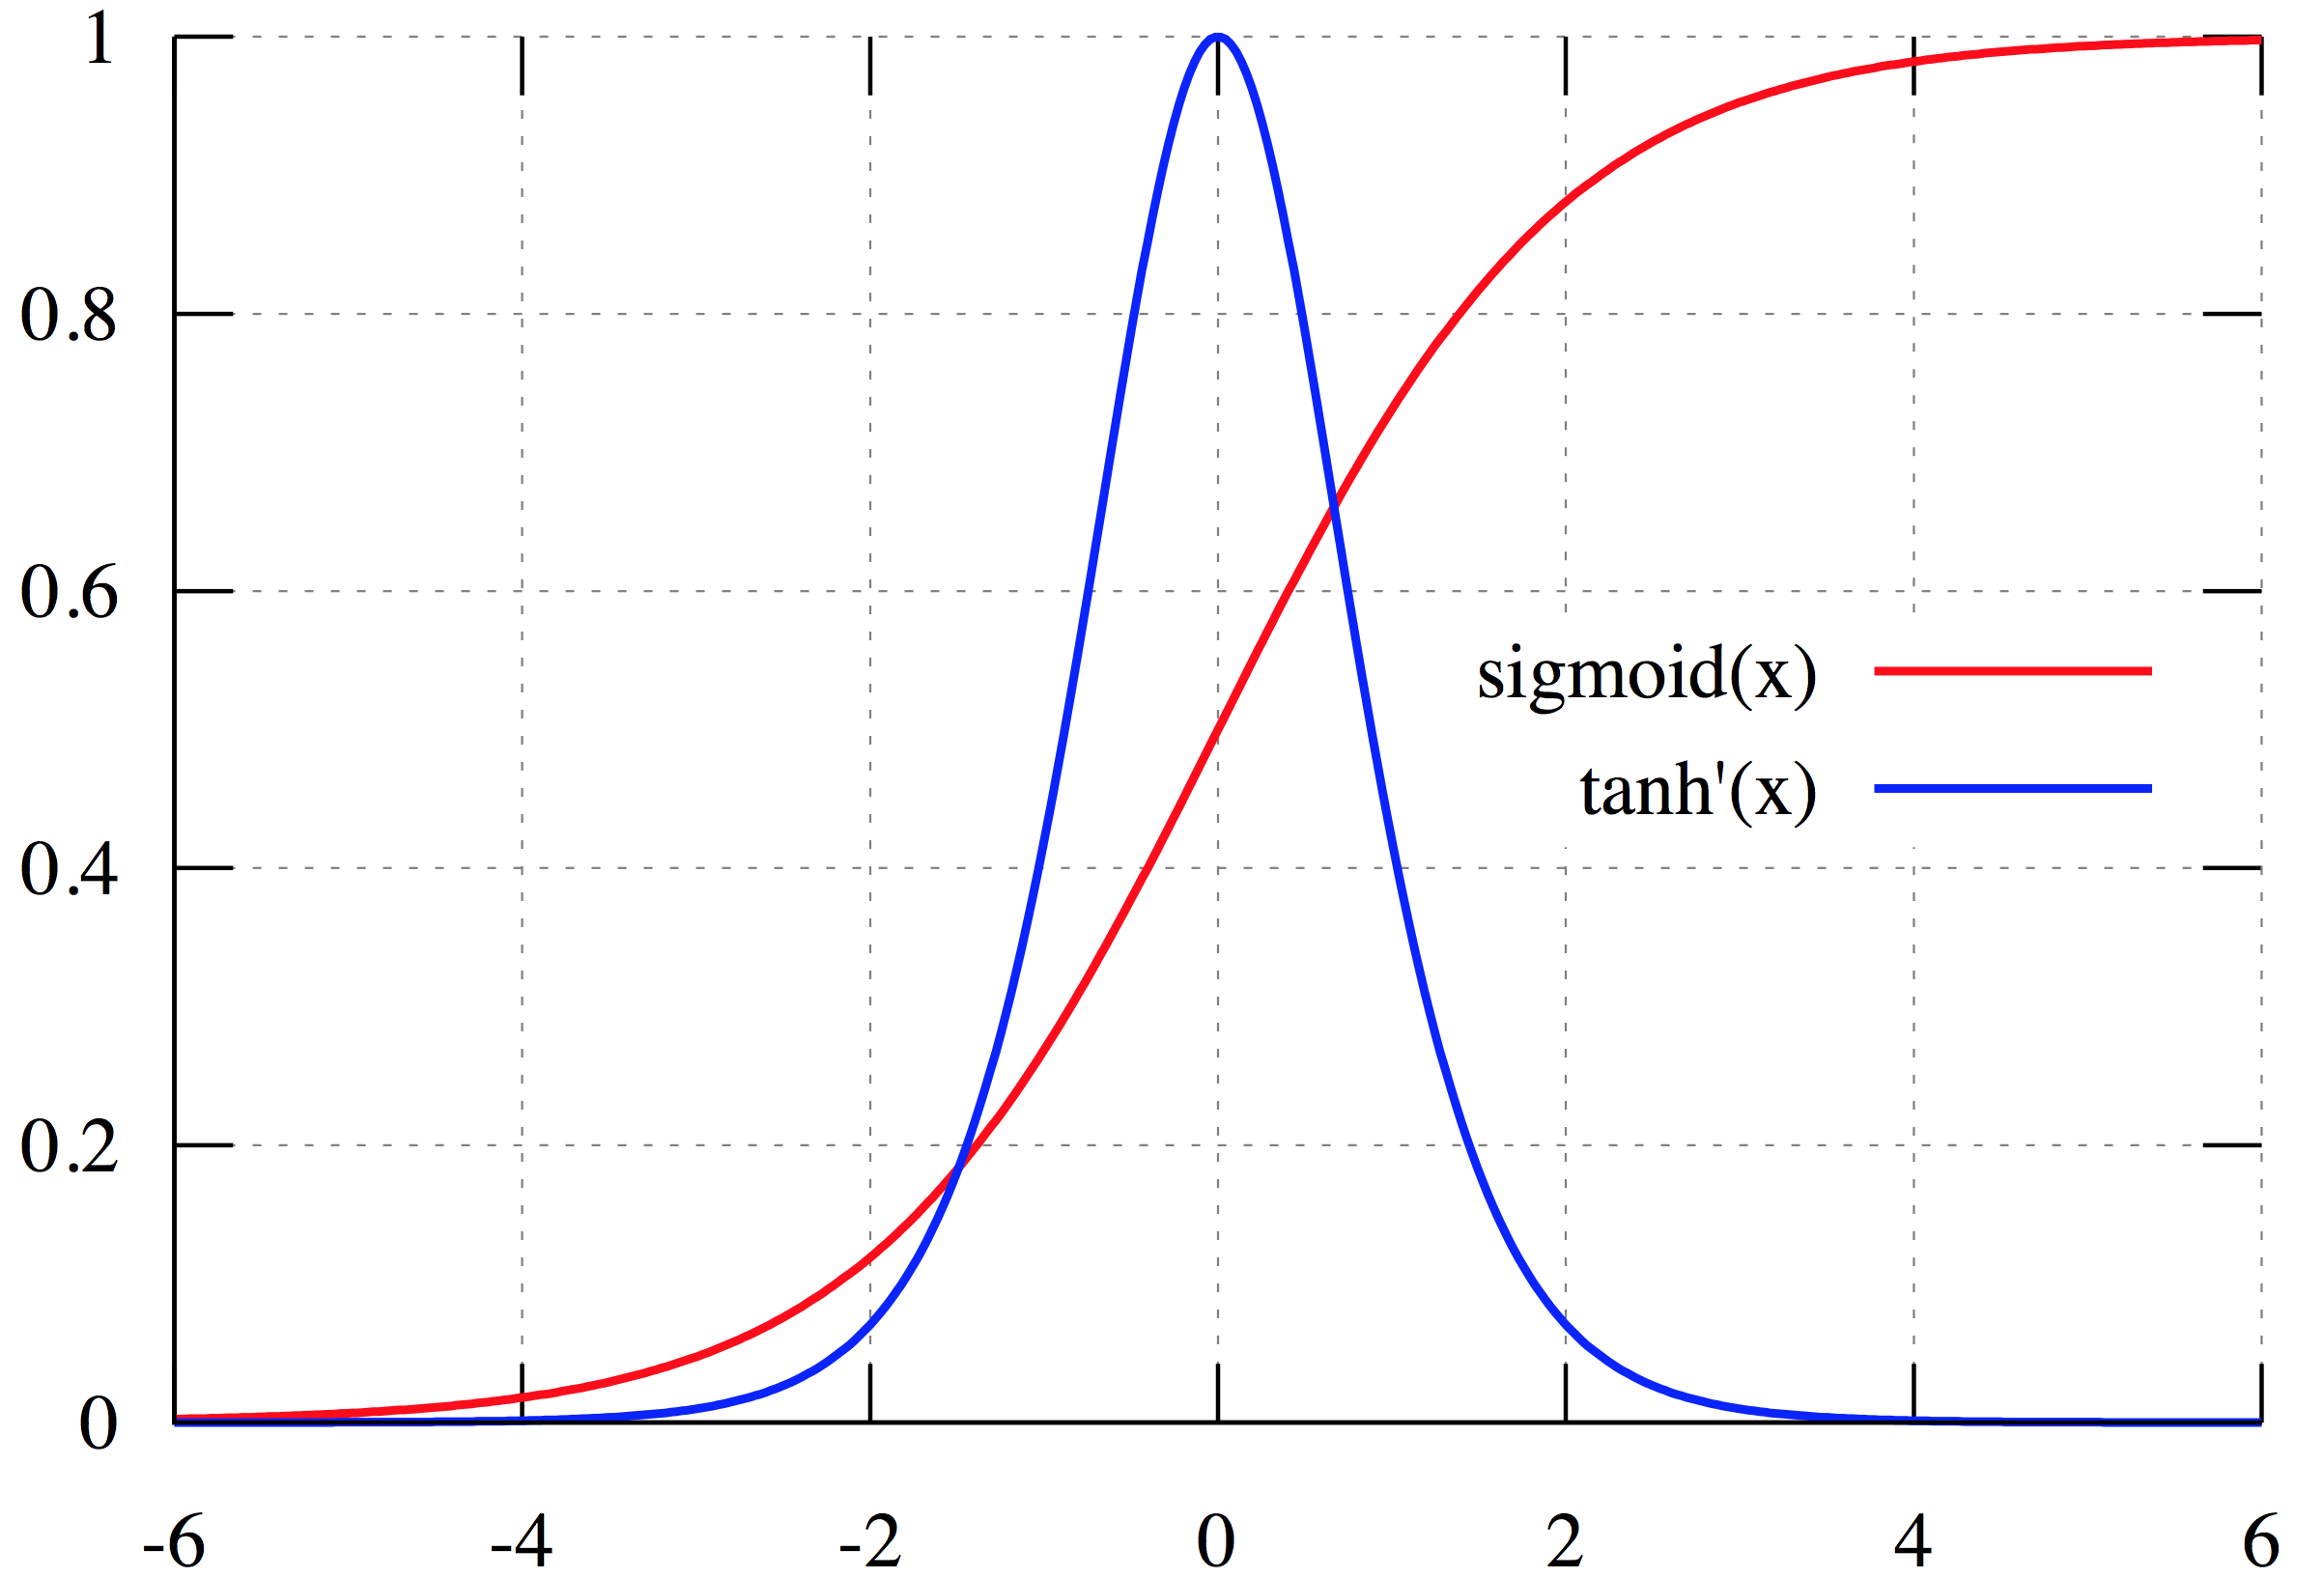
\includegraphics[width=0.65\textwidth, keepaspectratio]{compare}
	\caption{Compare the distribution of $sigmoid(x)$ and $tanh'(x)$}
	\label{fig:compare}
\end{figure}

\section{Implementation}
A prototype of RNN layer has been implemented in my github (\textbf{https://github.com/beekbin/simpleRNN}). 
In this implementation, to be able to be stacked by other sequence layer (for example, another RNN layer, or Pooling layer), the output of the RNN
layer is $Vh^{(t)}$, instead of $softmax(Vh^{(t)})$.  The $Softmax$ is implemented as a separate layer.


\section{Conclusion}
This essay has explained:
 \begin{itemize}
  \item The structure of RNN and LSTM;
  \item How to train RNN and LSTM with BPTT method;
  \item The gradient vanishing problem of RNN;
  \item How LSTM handles the gradient vanishing problem better than RNN.
 \end{itemize}

%\bibliographystyle{unsrt}
%\bibliography{bib}



\end{document}
